%%
% Copyright (c) 2017 - 2024, Pascal Wagler;
% Copyright (c) 2014 - 2024, John MacFarlane
%
% All rights reserved.
%
% Redistribution and use in source and binary forms, with or without
% modification, are permitted provided that the following conditions
% are met:
%
% - Redistributions of source code must retain the above copyright
% notice, this list of conditions and the following disclaimer.
%
% - Redistributions in binary form must reproduce the above copyright
% notice, this list of conditions and the following disclaimer in the
% documentation and/or other materials provided with the distribution.
%
% - Neither the name of John MacFarlane nor the names of other
% contributors may be used to endorse or promote products derived
% from this software without specific prior written permission.
%
% THIS SOFTWARE IS PROVIDED BY THE COPYRIGHT HOLDERS AND CONTRIBUTORS
% "AS IS" AND ANY EXPRESS OR IMPLIED WARRANTIES, INCLUDING, BUT NOT
% LIMITED TO, THE IMPLIED WARRANTIES OF MERCHANTABILITY AND FITNESS
% FOR A PARTICULAR PURPOSE ARE DISCLAIMED. IN NO EVENT SHALL THE
% COPYRIGHT OWNER OR CONTRIBUTORS BE LIABLE FOR ANY DIRECT, INDIRECT,
% INCIDENTAL, SPECIAL, EXEMPLARY, OR CONSEQUENTIAL DAMAGES (INCLUDING,
% BUT NOT LIMITED TO, PROCUREMENT OF SUBSTITUTE GOODS OR SERVICES;
% LOSS OF USE, DATA, OR PROFITS; OR BUSINESS INTERRUPTION) HOWEVER
% CAUSED AND ON ANY THEORY OF LIABILITY, WHETHER IN CONTRACT, STRICT
% LIABILITY, OR TORT (INCLUDING NEGLIGENCE OR OTHERWISE) ARISING IN
% ANY WAY OUT OF THE USE OF THIS SOFTWARE, EVEN IF ADVISED OF THE
% POSSIBILITY OF SUCH DAMAGE.
%%

%%
% This is the Eisvogel pandoc LaTeX template.
%
% For usage information and examples visit the official GitHub page:
% https://github.com/Wandmalfarbe/pandoc-latex-template
%%

% Options for packages loaded elsewhere
\PassOptionsToPackage{unicode}{hyperref}
\PassOptionsToPackage{hyphens}{url}
\PassOptionsToPackage{dvipsnames,svgnames,x11names,table}{xcolor}
%
\documentclass[
  paper=a4,
  ,captions=tableheading
]{scrartcl}
\usepackage{amsmath,amssymb}
% Use setspace anyway because we change the default line spacing.
% The spacing is changed early to affect the titlepage and the TOC.
\usepackage{setspace}
\setstretch{1.2}
\usepackage{iftex}
\ifPDFTeX
  \usepackage[T1]{fontenc}
  \usepackage[utf8]{inputenc}
  \usepackage{textcomp} % provide euro and other symbols
\else % if luatex or xetex
  \usepackage{unicode-math} % this also loads fontspec
  \defaultfontfeatures{Scale=MatchLowercase}
  \defaultfontfeatures[\rmfamily]{Ligatures=TeX,Scale=1}
\fi
\usepackage{lmodern}
\ifPDFTeX\else
  % xetex/luatex font selection
\fi
% Use upquote if available, for straight quotes in verbatim environments
\IfFileExists{upquote.sty}{\usepackage{upquote}}{}
\IfFileExists{microtype.sty}{% use microtype if available
  \usepackage[]{microtype}
  \UseMicrotypeSet[protrusion]{basicmath} % disable protrusion for tt fonts
}{}
\makeatletter
\@ifundefined{KOMAClassName}{% if non-KOMA class
  \IfFileExists{parskip.sty}{%
    \usepackage{parskip}
  }{% else
    \setlength{\parindent}{0pt}
    \setlength{\parskip}{6pt plus 2pt minus 1pt}}
}{% if KOMA class
  \KOMAoptions{parskip=half}}
\makeatother
\usepackage{xcolor}
\definecolor{default-linkcolor}{HTML}{A50000}
\definecolor{default-filecolor}{HTML}{A50000}
\definecolor{default-citecolor}{HTML}{4077C0}
\definecolor{default-urlcolor}{HTML}{4077C0}
\usepackage[top=1.3in,bottom=1in,left=0.6in,right=0.7in]{geometry}
\usepackage[export]{adjustbox}
\usepackage{graphicx}
\usepackage{etoolbox}
\BeforeBeginEnvironment{lstlisting}{\par\noindent\begin{minipage}{\linewidth}}
\AfterEndEnvironment{lstlisting}{\end{minipage}\par\addvspace{\topskip}}
\usepackage{longtable,booktabs,array}
\usepackage{calc} % for calculating minipage widths
% Correct order of tables after \paragraph or \subparagraph
\usepackage{etoolbox}
\makeatletter
\patchcmd\longtable{\par}{\if@noskipsec\mbox{}\fi\par}{}{}
\makeatother
% Allow footnotes in longtable head/foot
\IfFileExists{footnotehyper.sty}{\usepackage{footnotehyper}}{\usepackage{footnote}}
\makesavenoteenv{longtable}
% add backlinks to footnote references, cf. https://tex.stackexchange.com/questions/302266/make-footnote-clickable-both-ways
\usepackage{footnotebackref}
\usepackage{graphicx}
\makeatletter
\newsavebox\pandoc@box
\newcommand*\pandocbounded[1]{% scales image to fit in text height/width
  \sbox\pandoc@box{#1}%
  \Gscale@div\@tempa{\textheight}{\dimexpr\ht\pandoc@box+\dp\pandoc@box\relax}%
  \Gscale@div\@tempb{\linewidth}{\wd\pandoc@box}%
  \ifdim\@tempb\p@<\@tempa\p@\let\@tempa\@tempb\fi% select the smaller of both
  \ifdim\@tempa\p@<\p@\scalebox{\@tempa}{\usebox\pandoc@box}%
  \else\usebox{\pandoc@box}%
  \fi%
}
% Set default figure placement to htbp
% Make use of float-package and set default placement for figures to H.
% The option H means 'PUT IT HERE' (as  opposed to the standard h option which means 'You may put it here if you like').
\usepackage{float}
\floatplacement{figure}{H}
\makeatother
\setlength{\emergencystretch}{3em} % prevent overfull lines
\providecommand{\tightlist}{%
  \setlength{\itemsep}{0pt}\setlength{\parskip}{0pt}}
\setcounter{secnumdepth}{-\maxdimen} % remove section numbering
\ifLuaTeX
\usepackage[bidi=basic]{babel}
\else
\usepackage[bidi=default]{babel}
\fi
\babelprovide[main,import]{english}
% get rid of language-specific shorthands (see #6817):
\let\LanguageShortHands\languageshorthands
\def\languageshorthands#1{}
\makeatletter
\@ifpackageloaded{subfig}{}{\usepackage{subfig}}
\@ifpackageloaded{caption}{}{\usepackage{caption}}
\captionsetup[subfloat]{margin=0.5em}
\AtBeginDocument{%
\renewcommand*\figurename{Figura}
\renewcommand*\tablename{Tabla}
}
\AtBeginDocument{%
\renewcommand*\listfigurename{Lista de Figuras}
\renewcommand*\listtablename{Lista de Tablas}
}
\newcounter{pandoccrossref@subfigures@footnote@counter}
\newenvironment{pandoccrossrefsubfigures}{%
\setcounter{pandoccrossref@subfigures@footnote@counter}{0}
\begin{figure}\centering%
\gdef\global@pandoccrossref@subfigures@footnotes{}%
\DeclareRobustCommand{\footnote}[1]{\footnotemark%
\stepcounter{pandoccrossref@subfigures@footnote@counter}%
\ifx\global@pandoccrossref@subfigures@footnotes\empty%
\gdef\global@pandoccrossref@subfigures@footnotes{{##1}}%
\else%
\g@addto@macro\global@pandoccrossref@subfigures@footnotes{, {##1}}%
\fi}}%
{\end{figure}%
\addtocounter{footnote}{-\value{pandoccrossref@subfigures@footnote@counter}}
\@for\f:=\global@pandoccrossref@subfigures@footnotes\do{\stepcounter{footnote}\footnotetext{\f}}%
\gdef\global@pandoccrossref@subfigures@footnotes{}}
\@ifpackageloaded{float}{}{\usepackage{float}}
\floatstyle{ruled}
\@ifundefined{c@chapter}{\newfloat{codelisting}{h}{lop}}{\newfloat{codelisting}{h}{lop}[chapter]}
\floatname{codelisting}{Listing}
\newcommand*\listoflistings{\listof{codelisting}{Listas del Documento}}
\makeatother
\usepackage{bookmark}
\IfFileExists{xurl.sty}{\usepackage{xurl}}{} % add URL line breaks if available
\urlstyle{same}
\hypersetup{
  pdftitle={Certificación Operativa Plataforma de Software trii},
  pdfauthor={SoftProductiva.com},
  pdflang={en},
  pdfsubject={Implementación Proyecto},
  pdfkeywords={Rendimiento, Métodos pruebas, Pruebas software, QA},
  hidelinks,
  breaklinks=true,
  pdfcreator={LaTeX via pandoc with the Eisvogel template}}
\title{Certificación Operativa Plataforma de Software trii}
\usepackage{etoolbox}
\makeatletter
\providecommand{\subtitle}[1]{% add subtitle to \maketitle
  \apptocmd{\@title}{\par {\large #1 \par}}{}{}
}
\makeatother
\subtitle{Informe Técnico}
\author{SoftProductiva.com}
\date{2025-01-20}



%%
%% added
%%


%
% for the background color of the title page
%
\usepackage{pagecolor}
\usepackage{afterpage}
\usepackage{tikz}

%
% break urls
%
\PassOptionsToPackage{hyphens}{url}

%
% When using babel or polyglossia with biblatex, loading csquotes is recommended
% to ensure that quoted texts are typeset according to the rules of your main language.
%
\usepackage{csquotes}

%
% captions
%
\definecolor{caption-color}{HTML}{777777}
\usepackage[font={stretch=1.2}, textfont={color=caption-color}, position=top, skip=4mm, labelfont=bf, singlelinecheck=false, justification=raggedright]{caption}
\setcapindent{0em}

%
% blockquote
%
\definecolor{blockquote-border}{RGB}{221,221,221}
\definecolor{blockquote-text}{RGB}{119,119,119}
\usepackage{mdframed}
\newmdenv[rightline=false,bottomline=false,topline=false,linewidth=3pt,linecolor=blockquote-border,skipabove=\parskip]{customblockquote}
\renewenvironment{quote}{\begin{customblockquote}\list{}{\rightmargin=0em\leftmargin=0em}%
\item\relax\color{blockquote-text}\ignorespaces}{\unskip\unskip\endlist\end{customblockquote}}

%
% Source Sans Pro as the default font family
% Source Code Pro for monospace text
%
% 'default' option sets the default
% font family to Source Sans Pro, not \sfdefault.
%
\ifnum 0\ifxetex 1\fi\ifluatex 1\fi=0 % if pdftex
    \usepackage[default]{sourcesanspro}
  \usepackage{sourcecodepro}
  \else % if not pdftex
    \usepackage[default]{sourcesanspro}
  \usepackage{sourcecodepro}

  % XeLaTeX specific adjustments for straight quotes: https://tex.stackexchange.com/a/354887
  % This issue is already fixed (see https://github.com/silkeh/latex-sourcecodepro/pull/5) but the
  % fix is still unreleased.
  % TODO: Remove this workaround when the new version of sourcecodepro is released on CTAN.
  \ifxetex
    \makeatletter
    \defaultfontfeatures[\ttfamily]
      { Numbers   = \sourcecodepro@figurestyle,
        Scale     = \SourceCodePro@scale,
        Extension = .otf }
    \setmonofont
      [ UprightFont    = *-\sourcecodepro@regstyle,
        ItalicFont     = *-\sourcecodepro@regstyle It,
        BoldFont       = *-\sourcecodepro@boldstyle,
        BoldItalicFont = *-\sourcecodepro@boldstyle It ]
      {SourceCodePro}
    \makeatother
  \fi
  \fi

%
% heading color
%
\definecolor{heading-color}{RGB}{40,40,40}
\addtokomafont{section}{\color{heading-color}}
% When using the classes report, scrreprt, book,
% scrbook or memoir, uncomment the following line.
%\addtokomafont{chapter}{\color{heading-color}}

%
% variables for title, author and date
%
\usepackage{titling}
\title{Certificación Operativa Plataforma de Software trii}
\author{SoftProductiva.com}
\date{2025-01-20}

%
% tables
%

\definecolor{table-row-color}{HTML}{F5F5F5}
\definecolor{table-rule-color}{HTML}{999999}

%\arrayrulecolor{black!40}
\arrayrulecolor{table-rule-color}     % color of \toprule, \midrule, \bottomrule
\setlength\heavyrulewidth{0.3ex}      % thickness of \toprule, \bottomrule
\renewcommand{\arraystretch}{0.8}     % spacing (padding)


%
% remove paragraph indentation
%
\setlength{\parindent}{0pt}
\setlength{\parskip}{6pt plus 2pt minus 1pt}
\setlength{\emergencystretch}{3em}  % prevent overfull lines

%
%
% Listings
%
%


%
% header and footer
%
\usepackage[headsepline,footsepline]{scrlayer-scrpage}

\newpairofpagestyles{eisvogel-header-footer}{
  \clearpairofpagestyles
  \ihead*{2025-01-20}
  \chead*{}
  \ohead*{Certificación Operativa Plataforma de Software trii}
  \ifoot*{SoftProductiva.com}
  \cfoot*{}
  \ofoot*{\thepage}
  \addtokomafont{pageheadfoot}{\upshape}
}
\pagestyle{eisvogel-header-footer}



%%
%% end added
%%

%% change the default with of the images using \setkeys{Gin}{width=.8\linewidth}
\setkeys{Gin}{width=1\linewidth}

\begin{document}

%%
%% begin titlepage
%%
\begin{titlepage}
\newgeometry{top=2cm, right=4cm, bottom=3cm, left=4cm}
\tikz[remember picture,overlay] \node[inner sep=0pt] at (current page.center){
\includegraphics[width=\paperwidth,height=\paperheight]{include/background.pdf}};
\newcommand{\colorRule}[3][black]{\textcolor[HTML]{#1}{\rule{#2}{#3}}}
\begin{flushleft}
\noindent
\\[-1em]
\color[HTML]{5F5F5F}
\makebox[0pt][l]{\colorRule[360049]{1.3\textwidth}{4pt}}
\par
\noindent

% The titlepage with a background image has other text spacing and text size
{
  \setstretch{2}
  \vfill
  \vskip -8em
  \noindent {\huge \textbf{\textsf{Certificación Operativa Plataforma de
Software trii}}}
    \vskip 1em
  {\Large \textsf{Informe Técnico}}
    \vskip 2em
  \noindent {\Large \textsf{SoftProductiva.com} \vskip 0.6em \textsf{2025-01-20}}
  \vfill
}

\noindent

\includegraphics[width=60mm, right]{include/logo.png}


\end{flushleft}
\end{titlepage}
\restoregeometry
\pagenumbering{arabic}

%%
%% end titlepage
%%

% \maketitle


\section{Contenido}\label{sec:contenido}

\begin{itemize}
\tightlist
\item
  \hyperref[informaciuxf3n-del-documento]{Información del Documento}
\item
  \hyperref[informe-operativo-plataforma-de-software-]{Informe Operativo
  Plataforma de Software trii}
\item
  \hyperref[evaluaciuxf3n-del-rendimiento]{Evaluación del Rendimiento}
\item
  \hyperref[resultados-y-conclusiones-del-informe-de-rendimiento]{Resultados
  y Conclusiones del Informe de Rendimiento}
\item
  \hyperref[anexos-tuxe9cnicos]{Anexos Técnicos}
\item
  \hyperref[glosario]{Glosario}
\end{itemize}

\newpage

\section{Información del
Documento}\label{sec:informaciuxf3n-del-documento}

\subsection{Versión del Documento}\label{sec:versiuxf3n-del-documento}

\begin{quote}
\end{quote}

\subsection{Control de Cambios}\label{sec:control-de-cambios}

Historia de cambios del informe.

Versión actual: 1.f16bfa7 - Compilación para entrega:
observaciones-formato - c68b692 - Fri, 24 Jan 2025 19:51:47 +0000

Versiones Anteriores

1.a31c2e7 - todo - Thu, 23 Jan 2025 15:19:01 -0500

1.de1b246 - Compilación para entrega: observaciones-todo - 27d6a0e -
Thu, 23 Jan 2025 20:10:27 +0000

1.5b40f7c - cfg - Thu, 23 Jan 2025 15:09:30 -0500

1.37c623f - readm - Thu, 23 Jan 2025 15:07:46 -0500

\subsubsection{Realizado Por}\label{sec:realizado-por}

H. Wong, ing.

\subsubsection{Revisado Por}\label{sec:revisado-por}

(revisor), trii

\newpage

\section{Informe Operativo Plataforma de Software
trii}\label{sec:informe-operativo-plataforma-de-software-trii}

\subsection{Componentes del Informe de Rendimiento y Capacidad de la
Plataforma
trii}\label{sec:componentes-del-informe-de-rendimiento-y-capacidad-de-la-plataforma-trii}

\begin{quote}
\end{quote}

\begin{figure}
\centering
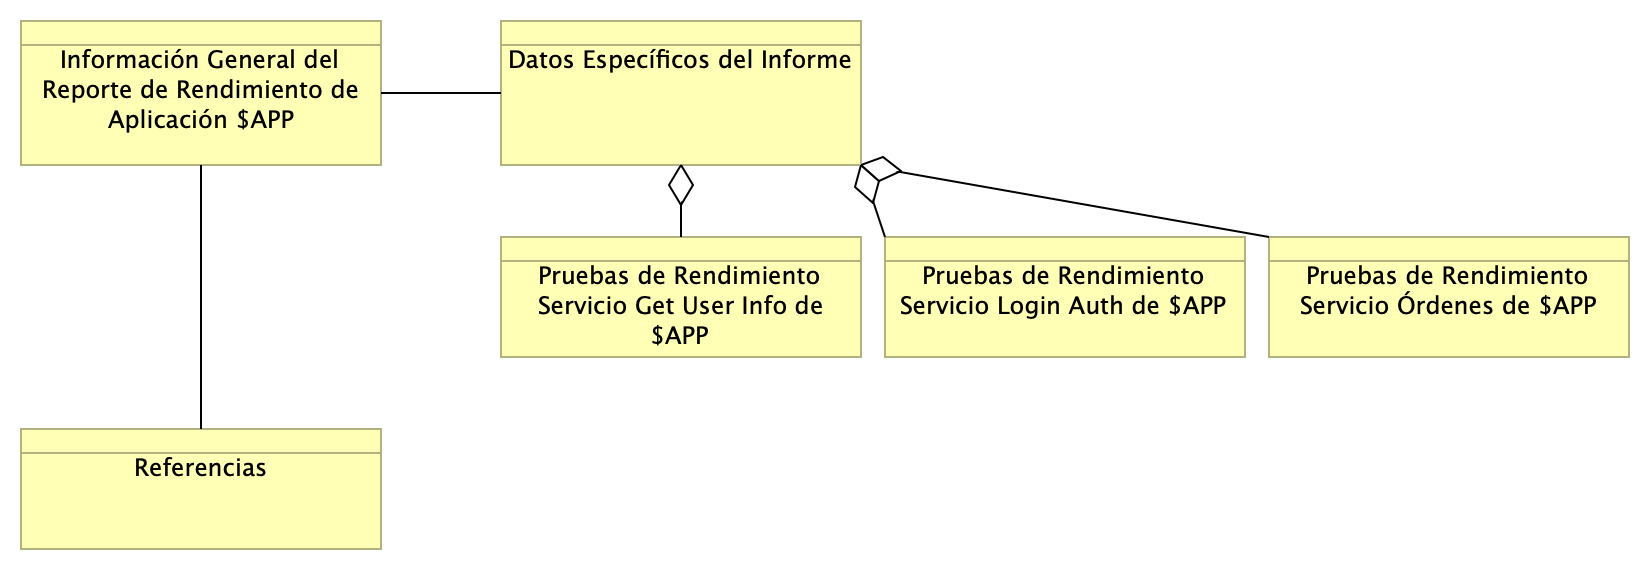
\includegraphics{images/05.b.Informe.png}
\caption{05.b.Informe. \emph{Fuente: Propuesta de certificación
operativa plataforma trii
(2025)}}\label{fig:id-04abc8f16f354757a52791da825e4049}
\end{figure}

\subsubsection{Información General del Reporte de Rendimiento de
Aplicación
trii}\label{sec:informaciuxf3n-general-del-reporte-de-rendimiento-de-aplicaciuxf3n-trii}

\begin{itemize}
\tightlist
\item
  Nombre de la Aplicación/Sistema Probado: Servicios de Órdenes, Auth, y
  User Info de la Aplicación trii
\item
  Versión de la Aplicación/Sistema: Versión 2025
\item
  Entorno de Pruebas: infraestructura en la nube, Google Cloud, 2nd
  generation machine series, General-purpose workloads E2 serie, CPU
  Intel. Tipo de equipo: highmem, 7-14 GB.
\item
  Fecha/Periodo de Pruebas: 15 de enero del 2025.
\item
  Objetivos de las Pruebas:

  \begin{itemize}
  \tightlist
  \item
    Encontrar la capacidad de los servicios Servicios Órdenes, Auth, y
    User Info de la Aplicación por separado en número máximo de
    operaciones o transacciones de los servicios por unidad de tiempo.
  \item
    Encontrar el nivel de estabilidad de los servicios Servicios
    Órdenes, Auth, y User Info (tensión) de la Aplicación.
  \item
    Dar pautas alrededor del estrés o tensión de los servicios Servicios
    Órdenes, Auth, y User Info de la Aplicación por separado para
    determinar la holgura respecto a la demanda esperada.
  \end{itemize}
\item
  Métricas Clave:

  \begin{itemize}
  \tightlist
  \item
    Capacidad (throughput) de los servicios Servicios Órdenes, Auth, y
    User Info
  \item
    Estrés (tensión) de los servicios Servicios Órdenes, Auth, y User
    Info
  \item
    Estabilidad (Uso de CPU) de los servicios Servicios Órdenes, Auth, y
    User Info Herramienta de Pruebas: K6, de Grafana Labs.
  \end{itemize}
\end{itemize}

\subsubsection{Datos Específicos del
Informe}\label{sec:datos-especuxedficos-del-informe}

Descripción detallada de los casos de uso o flujos de usuario simulados
de los servicios de Trii probados.

\subsubsection{Pruebas de Rendimiento Servicio Get User Info de
trii}\label{sec:pruebas-de-rendimiento-servicio-get-user-info-de-trii}

El servicio Get User Info (user info) obtiene datos de trabajo del
cliente previo a la orden. Requiere como mínimo actividades de
autenticación, y es responsable de alimentar al servicio Órdenes.

Carga de Usuarios: Cantidad de usuarios virtuales concurrentes
simulados, máximo 60. Duración de las Pruebas: Tiempo durante el cual se
ejecutaron las pruebas, mínimo 10 minutos.

\paragraph{Resultados Medidos}\label{sec:resultados-medidos}

Ejecución del escenario de pruebas de rendimiento descrito a
continuación del servicio Get User Info (user info) de la plataforma
trii.

\begin{quote}
Escenarios: (100.00\%) 1 scenario, 60 max VUs, 10m30s max duration
(incl.~graceful stop):

*default: Up to 60 looping VUs for 10m0s over 5 stages
(gracefulRampDown: 30s, gracefulStop 30s)

logged\_in\_successfully

is\_status\_200
\end{quote}

\begin{longtable}[]{@{}
  >{\raggedright\arraybackslash}p{(\columnwidth - 10\tabcolsep) * \real{0.2264}}
  >{\raggedright\arraybackslash}p{(\columnwidth - 10\tabcolsep) * \real{0.1509}}
  >{\raggedright\arraybackslash}p{(\columnwidth - 10\tabcolsep) * \real{0.1887}}
  >{\raggedright\arraybackslash}p{(\columnwidth - 10\tabcolsep) * \real{0.1509}}
  >{\raggedright\arraybackslash}p{(\columnwidth - 10\tabcolsep) * \real{0.1509}}
  >{\raggedright\arraybackslash}p{(\columnwidth - 10\tabcolsep) * \real{0.1321}}@{}}
\toprule\noalign{}
\endhead
\bottomrule\noalign{}
\endlastfoot
checks & 100.00\% & 57632 out of 57632 & & & \\
data\_received & 93 MB & 155 kB/s & & & \\
data\_sent & 14 MB & 23 kB/s & & & \\
http\_req\_blocked & avg=146.22µs & min=0s & p(95)=0s & p(90)=0s &
max=138.39ms \\
http\_req\_connecting & avg=51.45µs & min=0s & p(95)=0s & p(90)=0s &
max=2.39s \\
http\_req\_duration & avg=349.97ms & min=184.86ms & p(95)=849.58ms &
p(90)=786.74ms & max=2.39s \\
\{ expected\_response:tr & avg=349.97ms & min=184.86ms & p(95)=849.58ms
& p(90)=786.74ms & max=2.39s \\
http\_req\_failed & 0.00\% & 0/57632 & & & \\
http\_req\_receiving & avg=164.45µs & min=0s & p(95)=1.53ms &
p(90)=546.29µs & max=359.57ms \\
http\_req\_sending & avg=66.37µs & min=0s & p(95)=513.59µs & p(90)=0s &
max=2.41ms \\
http\_req\_tls\_handshaki & avg=138.25µs & min=0s & p(95)=0s & p(90)=0s
& max=2.39s \\
http\_req\_waiting & avg=349.74ms & min=184.86ms & p(95)=849.2ms &
p(90)=786.62ms & max=2.39s \\
http\_reqs & 57632 & 960.294772/s & & & \\
iteration\_duration & avg=708.46ms & min=293.83ms & p(95)=1.15s &
p(90)=987.68ms & max=2.52s \\
iterations & 28816 & 479.944772/s & & & \\
login\_response\_times & avg=136.021551 & min=104 & p(95)=177 &
p(90)=163 & max=296 \\
login\_success\_rate & 100.00\% & 28816 out of 28816 & & & \\
requests\_sent & 57632 & 95.929047/s & & & \\
user\_info\_response\_tim & avg=564.321835 & min=178 & p(95)=1027 &
p(90)=849 & max=2399 \\
user\_info\_success\_rate & 100.00\% & 28816 out of 28816 & & & \\
vus & 59 & min=1 & & & \\
vus\_max & 60 & min=60 & & & \\
\end{longtable}

\begin{quote}
Running (10m00.8s), 00/60 VUs, 28816 completed and 0 interrupted
iterations

default OK: 00/60 VUs 10m0s
\end{quote}

\paragraph{Valores Numéricos}\label{sec:valores-numuxe9ricos}

Promedio por transacción, tiempo máximo, mínimo, y percentiles de las
métricas. Tomado del mayor entre http\_req\_duration e
iteration\_duration.

\begin{quote}
Tiempo máximo de la transacción (iteración): max=2.52s

Tiempo promedio: avg=708.46ms

Tiempo mínimo: min=293.83ms

Percentiles 90 y 95 duración iteración: p(90)=987.68ms; p(95)=1.15s

Cantidad de transacciones/segundo (capacidad o throughput): 57632 total;
95.929047/s

Estabilidad o Tasa de éxito de transacción (promedio entre dos
servicios, login y user\_info): 100.00\%; 28816 de 28816 procesados
\end{quote}

\paragraph{Desviaciones}\label{sec:desviaciones}

Comportamiento inesperado o desviaciones significativas de los valores
esperados.

Con base en los tiempos de latencia cercanos al tiempo de transacción y
la alta la tasa de éxito de transacción, no hay evidencia de
desviaciones.

\begin{quote}
Latencia promedio: avg=349.74ms

Latencia máxima: max=2.39s

Estabilidad o Tasa de éxito de transacción (promedio entre dos
servicios, login y user\_info): 100.00\%; 28816 de 28816 procesados
\end{quote}

\paragraph{Análisis de Cuellos de
Botella}\label{sec:anuxe1lisis-de-cuellos-de-botella}

Identificación de componentes o procesos que limitaron el rendimiento.

Con base en los tiempos de rendimiento (capacidad o throughput) y la
alta la tasa de éxito de la transacción, no es posible señalar un cuello
de botella.

\begin{quote}
Cantidad de transacciones/segundo (capacidad o throughput iteración):
57632 total; 95.929047/s

Estabilidad o Tasa de éxito de transacción (promedio entre dos
servicios, login y user\_info): 100.00\%; 28816 de 28816 procesados
\end{quote}

\paragraph{Limitaciones}\label{sec:limitaciones}

Con base en las 28816 iteraciones completadas y 0 interrumpidas, no hubo
limitaciones o condiciones conocidas durante las pruebas que podrían
afectar los resultados.

\begin{quote}
Calidad de la prueba: 28816 iteraciones completadas; 0 interrumpidas
\end{quote}

\subsubsection{Pruebas de Rendimiento Servicio Login Auth de
trii}\label{sec:pruebas-de-rendimiento-servicio-login-auth-de-trii}

El servicio Login (auth) es responsable de dar inicio a una sesión de
trabajo de un cliente trii. Realiza como mínimo la provisión de datos
necesarios a otros servicios respecto de la verificación y creación de
una sesión de trabajo válida.

Carga de Usuarios: Cantidad de usuarios virtuales concurrentes
simulados, máximo 60. Duración de las Pruebas: Tiempo durante el cual se
ejecutaron las pruebas, mínimo 10 minutos.

\paragraph{Resultados Medidos}\label{sec:resultados-medidos-1}

Ejecución del escenario de pruebas de rendimiento descrito a
continuación del servicio Login (auth) de la plataforma trii.

\begin{quote}
Escenarios: (100.00\%) 1 scenario, 60 max VUs, 10m30s max duration
(incl.~graceful stop):

*default: Up to 60 looping VUs for 10m0s over 5 stages
(gracefulRampDown: 30s, gracefulStop: 30s)

logged\_in\_successfully
\end{quote}

\begin{longtable}[]{@{}
  >{\raggedright\arraybackslash}p{(\columnwidth - 10\tabcolsep) * \real{0.2294}}
  >{\raggedright\arraybackslash}p{(\columnwidth - 10\tabcolsep) * \real{0.1560}}
  >{\raggedright\arraybackslash}p{(\columnwidth - 10\tabcolsep) * \real{0.2018}}
  >{\raggedright\arraybackslash}p{(\columnwidth - 10\tabcolsep) * \real{0.1468}}
  >{\raggedright\arraybackslash}p{(\columnwidth - 10\tabcolsep) * \real{0.1468}}
  >{\raggedright\arraybackslash}p{(\columnwidth - 10\tabcolsep) * \real{0.1193}}@{}}
\toprule\noalign{}
\endhead
\bottomrule\noalign{}
\endlastfoot
checks & 100.00\% & 113667 out of 113667 & & & \\
data\_received & 57 MB & 93 kB/s & & & \\
data\_sent & 21 MB & 35 kB/s & & & \\
http\_req\_blocked & avg=37.58µs & min=9s & p(95)=0s & p(90)=0s &
max=92.67ms \\
http\_req\_connecting & avg=1.35µs & min=0s & p(95)=0s & p(90)=0s &
max=3.66ms \\
http\_req\_duration & avg=177.22ms & min=105.54ms & p(95)=315.41ms &
p(90)=261.69ms & max=3.67s \\
\{ expected\_response: tr & avg=177.22ms & min=105.54ms & p(95)=315.41ms
& p(90)=261.69ms & max=3.67s \\
http\_req\_failed & 0.00\% & 0 out of 113677 & & & \\
http\_req\_receiving & avg=82.42µs & min=9s & p(95)=150.5µs &
p(90)=55.2µs & max=71.71ms \\
http\_req\_sending & avg=82.9µs & min=9s & p(95)=569.37µs & p(90)=0s &
max=2.76ms \\
http\_req\_tls\_handshakin & avg=36.3µs & min=0s & p(95)=0s & p(90)=0s &
max=87.34ms \\
http\_req\_waiting & avg=176.98ms & min=105.54ms & p(95)=315.16ms &
p(90)=261.41ms & max=3.67s \\
http\_reqs & 113677 & 189.19272/s & & & \\
iteration\_duration & avg=177.38ms & min=105.71ms & p(95)=315.52ms &
p(90)=261.84ms & max=3.67s \\
iterations & 113677 & 189.19272/s & & & \\
login\_response\_times & avg=177.3086641 & min=105 & p(95)=316 &
p(90)=262 & max=3675 \\
login\_success\_rate & 100.00\% & 113677 out of 113677 & & & \\
requests\_sent & 113677 & 189.19272/s & & & \\
vus & 59 & min=1 & & & \\
vus\_max & 60 & min=60 & & & \\
\end{longtable}

\begin{quote}
Running (10m00.2s), 00/60 VUs, 1136777 completed and 0 interrupted
iterations

default OK: 00/60 VUs 10m0s
\end{quote}

\paragraph{Valores Numéricos}\label{sec:valores-numuxe9ricos-1}

Promedio por transacción, tiempo máximo, mínimo, y percentiles de las
métricas. Tomado del mayor entre http\_req\_duration e
iteration\_duration.

\begin{quote}
Tiempo máximo de la transacción (iteración): max=3.67s

Tiempo promedio: avg=177.38ms

Tiempo mínimo: min=105.71ms

Percentiles 90 y 95 duración iteración: p(90)=261.84ms; p(95)=315.52ms

Cantidad de transacciones/segundo (capacidad o throughput): 113677
total; 189.19272/s

Estabilidad o Tasa de éxito de transacción: 100.00\%; 113677 de 113677
procesados
\end{quote}

Nota: el tiempo máximo de transacción, si bien es mayor a 3s, es aún
eficiente debido al tipo de transacción, en este caso de autenticación,
que no compromete al valor del negocio de trii. Más aún, que el promedio
en este caso no es representativo de la muestra, como sí lo es el valor
del percentil 95: p(95)=315.52ms por transacción.

\paragraph{Desviaciones}\label{sec:desviaciones-1}

Comportamiento inesperado o desviaciones significativas de los valores
esperados.

Con base en los tiempos de latencia cercanos al tiempo de transacción y
la alta la tasa de éxito de transacción, no hay evidencia de
desviaciones.

\begin{quote}
Latencia promedio: avg=176.98ms

Latencia máxima: max=3.67s; p(95)=315.52ms

Estabilidad o Tasa de éxito de transacción: 100.00\%; 113677 de 113677
procesados
\end{quote}

Nota: el tiempo máximo de latencia, si bien es mayor a 3s, es aún
eficiente debido al tipo de transacción, en este caso de autenticación,
que no compromete al negocio de trii. Más aún, que el promedio en este
caso no es representativo de la muestra, como sí lo es el valor del
percentil 95: p(95)=315.52ms por transacción.

\paragraph{Análisis de Cuellos de
Botella}\label{sec:anuxe1lisis-de-cuellos-de-botella-1}

Identificación de componentes o procesos que limitaron el rendimiento.

\begin{quote}
Latencia máxima: max=3.67s

Latencia promedio: avg=176.98ms
\end{quote}

Nota: con base en la diferencia entre la latencia máxima y la promedio
es posible señalar afectación de recursos de la transacción debido a la
concurrencia de los VU (60, para este escenario).

Aún así, por los tiempos de rendimiento (capacidad o throughput) y la
alta la tasa de éxito de la transacción, no es posible señalar que la
posibilidad del cuello de botella en el servicio Auth sea incidente en
el negocio de trii. Dicho de otra manera, la transacción es resiliente a
pesar de las afectaciones por concurrencia.

\begin{quote}
Cantidad de transacciones/segundo (capacidad o throughput): 113677
total; 189.19272/s

Estabilidad o Tasa de éxito de transacción: 100.00\%; 113677 de 113677
procesados
\end{quote}

\paragraph{Limitaciones}\label{sec:limitaciones-1}

\begin{quote}
No hubo limitaciones o condiciones conocidas durante las pruebas que
podrían afectar los resultados.
\end{quote}

\subsubsection{Pruebas de Rendimiento Servicio Órdenes de
trii}\label{sec:pruebas-de-rendimiento-servicio-uxf3rdenes-de-trii}

El servicio Órdenes es el más relevante para el negocio de trii. Realiza
como mínimo actividades de creación de una orden de negocio, que es la
entidad de información superlativa de la plataforma.

Carga de Usuarios: Cantidad de usuarios virtuales concurrentes
simulados, máximo 60. Duración de las Pruebas: Tiempo durante el cual se
ejecutaron las pruebas, mínimo 10 minutos.

\paragraph{Resultados Medidos}\label{sec:resultados-medidos-2}

Ejecución del escenario de pruebas de rendimiento descrito a
continuación del servicio Órdenes de la plataforma trii.

\begin{quote}
Escenarios: (100.00\%) 1 scenario, 60 max VUs, 10m30s max duration
(incl.~graceful stop):

*default: Up to 60 looping VUs for 10m0s over 5 stages
(gracefulRampDown: 30s, gracefulStop: 30s)

logged\_in\_successfully

is\_status\_200

86\%: OK 9881 / ERR 1506
\end{quote}

\begin{longtable}[]{@{}
  >{\raggedright\arraybackslash}p{(\columnwidth - 10\tabcolsep) * \real{0.2308}}
  >{\raggedright\arraybackslash}p{(\columnwidth - 10\tabcolsep) * \real{0.1635}}
  >{\raggedright\arraybackslash}p{(\columnwidth - 10\tabcolsep) * \real{0.1923}}
  >{\raggedright\arraybackslash}p{(\columnwidth - 10\tabcolsep) * \real{0.1538}}
  >{\raggedright\arraybackslash}p{(\columnwidth - 10\tabcolsep) * \real{0.1346}}
  >{\raggedright\arraybackslash}p{(\columnwidth - 10\tabcolsep) * \real{0.1250}}@{}}
\toprule\noalign{}
\endhead
\bottomrule\noalign{}
\endlastfoot
checks & 93.38\% & 21268 out of 22774 & & & \\
data\_received & 11 MB & 19 kB/s & & & \\
data\_sent & 7.5 MB & 13 kB/s & & & \\
failed\_transactions & avg=1 & min=1 & p(95)=1 & p(90)=1 & max=1 \\
http\_req\_blocked & avg=359.1µs & min=0s & p(95)=8s & p(90)=8s &
max=98.53ms \\
http\_req\_connecting & avg=216.56µs & min=0s & p(95)=0s & p(90)=0s &
max=16.6s \\
http\_req\_duration & avg=888.53ms & min=197.84ms & p(95)=2.7s &
p(90)=2.21s & max=16.6s \\
\{ http\_req\_response:tr & avg=216.56µs & min=0s & p(95)=2.75s &
p(90)=2.26s & max=16.6s \\
http\_req\_failed & 0.61\% & 1506 out of 22774 & & & \\
http\_req\_receiving & avg=130.7µs & min=0s & p(95)=573.02µs & p(90)=8s
& max=1.99ms \\
http\_req\_sending & avg=78.33µs & min=0s & p(95)=573.02µs & p(90)=8s &
max=1.99ms \\
http\_req\_tls\_handshaki & avg=284.26µs & min=0s & p(95)=0s & p(90)=0s
& max=16.58s \\
http\_req\_waiting & avg=888.32ms & min=197.84ms & p(95)=2.7s &
p(90)=2.21s & max=16.6s \\
http\_reqs & 2052/s & 22774 & & & \\
iteration\_duration & avg=1.77s & min=419.76ms & p(95)=3.31s &
p(90)=2.83s & max=16.74s \\
iterations & 11387 & 1025.73/s & & & \\
login\_response\_times & avg=130.558435 & min=197 & p(95)=157 &
p(90)=146 & max=333 \\
login\_success\_rate & 188.889.111147 & 2.111147 & & & \\
requests\_sent & 22774 & 77.71065/s & & & \\
successful\_transaction & 9881 & 16.36504/s & & & \\
transaction\_response\_t & avg=1647.048309 & min=388 & p(95)=3178.7 &
p(90)=2705.8 & max=16658 \\
vus & 60 & min=60 & & & max=60 \\
vus\_max & 60 & min=60 & & & max=60 \\
\end{longtable}

\begin{quote}
Running (10m03.8s), 00/60 VUs, 11387 completed and 0 interrupted
iterations

default OK: 00/60 VUs 10m0s
\end{quote}

Nota: el estado 200 (petición HTML exitosa) en las transacciones del
servicio Órdenes representa además el estado de negocio; es decir, una
transacción correctamente procesada por el sistema, y aceptada por las
reglas de negocio, retorna el estado HTTP 200 en caso que no haya
ocurrido una excepción de negocio. Esto es lo mismo decir que las
transacciones con estado HTML distintas del 200 resultantes en este
escenario de prueba, más precisamente fueron procesadas exitosamente por
el sistema (procesadas sin fallos de sistema evidenciado en logs) aún
cuando hubiesen caído en una regla o excepción de negocio.

\paragraph{Valores Numéricos}\label{sec:valores-numuxe9ricos-2}

Promedio por transacción, tiempo máximo, mínimo, y percentiles de las
métricas. Tomado del mayor entre http\_req\_duration e
iteration\_duration.

\begin{quote}
Tiempo máximo de la transacción (iteración): max=16.74s; avg
p(95/90)=4.49s

Tiempo promedio: avg=1.77s; p(95)=3.31s

Tiempo mínimo: min=419.76ms

Percentiles 90 y 95 duración iteración: p(90)=2.83s; p(95)=3.31s

Cantidad de transacciones/segundo (capacidad o throughput): 22774 total;
16.36504/s

Estabilidad o Tasa de éxito de transacción (iteración): 100.00\%; 11387
de 11387. De las cuales 86.00\% Órdenes de Negocio (9881 de 11387)
exitosas
\end{quote}

Nota: el estado 200 (petición HTML exitosa) en las transacciones del
servicio Órdenes representa además el estado de negocio; es decir, una
transacción correctamente procesada por el sistema, y aceptada por las
reglas de negocio, retorna el estado HTTP 200 en caso que no haya
ocurrido una excepción de negocio. Esto es lo mismo decir que las
transacciones con estado HTML distintas del 200 resultantes en este
escenario de prueba, fueron procesadas exitosamente por el sistema
(procesadas sin fallos de sistema evidenciado en logs) aún cuando
hubiesen caído en una regla o excepción de negocio.

Nota: debido a la diferencia entre el tiempo promedio de la transacción
y el percentil 95, el tiempo máximo de transacción no es representativo
de la muestra. Tomaremos como valor máximo de la transacción de Órdenes
al promedio de los percentiles 90 y 95, que es p(95/90)=4.49s.

Nota: el tiempo máximo de transacción (iteración) de Órdenes, si bien es
mayor a 3s, es aún eficiente debido a la complejidad de la transacción y
que no está comprometiendo al negocio de trii evidenciado en la
estabilidad del 100\% de este servicio y en el percentil 95 de duración,
que sí es representativo, y es de p(95)=3.31s por transacción.

\paragraph{Desviaciones}\label{sec:desviaciones-2}

Comportamiento inesperado o desviaciones significativas de los valores
esperados.

Con base en los tiempos de latencia cercanos al tiempo de transacción y
la alta la tasa de éxito de transacción, no hay evidencia de
desviaciones.

\begin{quote}
Latencia promedio: avg=888.32ms; p(95)=2.7s

Latencia máxima: max=16.6s; avg p(95/90)=3.8s

Estabilidad o Tasa de éxito de transacción (iteración): 100.00\%; 11387
de 11387. De las cuales 86.00\% Órdenes de Negocio (9881 de 11387)
exitosas
\end{quote}

Nota: Debido a la diferencia entre la latencia promedio y su percentil
95, el tiempo máximo de latencia por transacción no es representativo de
la muestra. Tomaremos como valor máximo de la latencia de Órdenes al
promedio de los percentiles 90 y 95, que es p(95/90)=3.8s.

Nota: el tiempo máximo de latencia, si bien es mayor a 3s, es aún
eficiente debido a la complejidad de la transacción Órdenes y no está
comprometiendo al negocio de trii evidenciado en la estabilidad del
100\% de este servicio y en el percentil 95 de latencia, que sí es
representativo, y es de p(95)=2.7s por transacción.

\paragraph{Análisis de Cuellos de
Botella}\label{sec:anuxe1lisis-de-cuellos-de-botella-2}

Identificación de componentes o procesos que limitaron el rendimiento.

\begin{quote}
Latencia máxima: max=16.6s; avg p(95/90)=3.8s

Latencia promedio: avg=888.32ms; p(95)=2.7s
\end{quote}

Nota: con base en la diferencia entre la latencia máxima y la promedio
existe alta posibilidad de recursos de la transacción Órdenes afectados
por la concurrencia de los VU (60, para este escenario).

Aún así, los tiempos de rendimiento (capacidad o throughput),
16.36504/s, y la tasa de éxito de la transacción, no es posible señalar
que la posibilidad del cuello de botella esté afectando al negocio de
trii. Dicho de otra manera, la transacción Órdenes es resiliente a pesar
de las afectaciones por concurrencia.

\begin{quote}
Cantidad de transacciones/segundo (capacidad o throughput): 22774 total;
16.36504/s

Estabilidad o Tasa de éxito de transacción (iteración): 100.00\%; 11387
de 11387. De las cuales 86.00\% Órdenes de Negocio (9881 de 11387)
exitosas
\end{quote}

\paragraph{Limitaciones}\label{sec:limitaciones-2}

En este escenario existieron limitaciones o condiciones conocidas del
balance de Órdenes durante las pruebas que afectaron los resultados de
las métricas de transacción exitosa.

\begin{quote}
is\_status\_200

86\%: OK 9881 / ERR 1506

Estabilidad o Tasa de éxito de transacción (iteración): 100.00\%; 11387
de 11387. De las cuales 86.00\% Órdenes de Negocio (9881 de 11387)
exitosas
\end{quote}

El estado 200 (petición HTML exitosa) en las transacciones del servicio
Órdenes representa además el estado de negocio; es decir, una
transacción correctamente procesada por el sistema, y aceptada por las
reglas de negocio, retorna el estado HTTP 200 en caso que no haya
ocurrido una excepción de negocio. Esto es lo mismo decir que las
transacciones con estado HTML distintas del 200 resultantes en este
escenario de prueba, fueron procesadas exitosamente por el sistema
(procesadas sin fallos de sistema evidenciado en logs) aún cuando
hubiesen caído en una regla o excepción de negocio.

\subsubsection{Referencias}\label{sec:referencias}

\begin{enumerate}
\def\labelenumi{\arabic{enumi}.}
\item
  Google (2025). Machine families resource and comparison guide.

  (Web) https://cloud.google.com/compute/docs/machine-resource
\item
  Grafana Labs (2025). Technical documentation. Grafana Cloud.

  (Web) https://grafana.com/docs/k6/latest/
\item
  Heusser M. (Sep 2019). How to achieve speedy application response
  times.

  (Web)
  https://www.techtarget.com/searchsoftwarequality/tip/Acceptable-application-response-times-vs-industry-standard
\item
  Nielsen, J. (1993). Usability Engineering. Response Times: The 3
  Important Limits.

  (Web)
  https://www.nngroup.com/articles/response-times-3-important-limits/
\end{enumerate}

\newpage

\section{Evaluación del
Rendimiento}\label{sec:evaluaciuxf3n-del-rendimiento}

\subsection{Método de Evaluación del Rendimiento Actual de
trii}\label{sec:muxe9todo-de-evaluaciuxf3n-del-rendimiento-actual-de-trii}

\begin{quote}
\end{quote}

\subsubsection{Criterios de Evaluación del Rendimiento
Actual}\label{sec:criterios-de-evaluaciuxf3n-del-rendimiento-actual}

\section{Multiline Text Table}\label{sec:multiline-text-table}

\begin{longtable}[]{@{}
  >{\raggedright\arraybackslash}p{(\columnwidth - 4\tabcolsep) * \real{0.3267}}
  >{\raggedright\arraybackslash}p{(\columnwidth - 4\tabcolsep) * \real{0.2673}}
  >{\raggedright\arraybackslash}p{(\columnwidth - 4\tabcolsep) * \real{0.4059}}@{}}
\toprule\noalign{}
\begin{minipage}[b]{\linewidth}\raggedright
Column 1
\end{minipage} & \begin{minipage}[b]{\linewidth}\raggedright
Column 2
\end{minipage} & \begin{minipage}[b]{\linewidth}\raggedright
Column 3
\end{minipage} \\
\midrule\noalign{}
\endhead
\bottomrule\noalign{}
\endlastfoot
First line of text & This is a single line of text & Line 1 of textLine
2 of textLine 3 of textLine 4 of text \\
Text in the first columnMore text in the first column & First line of
textSecond line of text & Just a single line \\
MultilineTextHere & Another line of text & Line 1 of textLine 2 of
textLine 3 of text \\
\end{longtable}

\newpage

\section{Resultados y Conclusiones del Informe de
Rendimiento}\label{sec:resultados-y-conclusiones-del-informe-de-rendimiento}

\subsection{Análisis de Resultados del Rendimiento y
Capacidad}\label{sec:anuxe1lisis-de-resultados-del-rendimiento-y-capacidad}

\begin{quote}
\end{quote}

\subsubsection{Resumen y Puntos Sobresalientes de los
Resultados}\label{sec:resumen-y-puntos-sobresalientes-de-los-resultados}

\begin{enumerate}
\def\labelenumi{\arabic{enumi}.}
\tightlist
\item
  Todos los servicios probados (auth, user\_info, fee y órdenes) pasaron
  los criterios de aceptación de estabilidad, tiempo de respuesta, y
  capacidad de cómputo (throughput). Pag. 14, Informe Técnico
\item
  El análisis de latencia del servicio de Órdenes indica una alta
  posibilidad de que exista un cuello botella, pero no afecta la
  estabilidad del servicio: cero (0) fallas en registro de actividad del
  sistema. Pág. 11, Informe Técnico; razón por la cual
\item
  El servicio de órdenes requirió del ajuste en el criterio de
  aceptación \emph{tiempo de respuesta}: quedó en 4.5s. Pág. 10, Informe
  Técnico
\item
  La conclusión general del rendimiento de trii actual, `como está', sin
  inversión de capacidad, presenta holgura del 4x. Es decir, sin cambios
  en el plan de capacidad trii puede crecer un 400\% del rendimiento
  actual. Pág. 15, Informe Técnico
\end{enumerate}

\subsubsection{Compilación de Resultado de las Pruebas de
Rendimiento}\label{sec:compilaciuxf3n-de-resultado-de-las-pruebas-de-rendimiento}

\begin{longtable}[]{@{}
  >{\raggedright\arraybackslash}p{(\columnwidth - 4\tabcolsep) * \real{0.1053}}
  >{\raggedright\arraybackslash}p{(\columnwidth - 4\tabcolsep) * \real{0.4105}}
  >{\raggedright\arraybackslash}p{(\columnwidth - 4\tabcolsep) * \real{0.4842}}@{}}
\toprule\noalign{}
\begin{minipage}[b]{\linewidth}\raggedright
Prueba
\end{minipage} & \begin{minipage}[b]{\linewidth}\raggedright
Criterio de Aceptación
\end{minipage} & \begin{minipage}[b]{\linewidth}\raggedright
Resultado
\end{minipage} \\
\midrule\noalign{}
\endhead
\bottomrule\noalign{}
\endlastfoot
Login & Percentil de peticiones exitosas 99.9 & Estabilidad o Tasa de
éxito de transacción: 100.00\%; 113677 de 113677 procesados \\
Login & Tiempo de respuesta max 4 seg. & Tiempo máximo de la transacción
(iteración): max=3.67s \\
Login & Tasa procesamiento (throughput), 2500 transacciones por hora y
40 por minuto & Cantidad de transacciones/segundo (capacidad o
throughput): 113677 total; 189.19272/s \\
Get user info & Percentil de peticiones exitosas 99.9 & Estabilidad o
Tasa de éxito de transacción: 100.00\%; 28816 de 28816 procesados \\
Get user info & Tiempo de respuesta max 4 seg. & Tiempo máximo de la
transacción (iteración): max=2.52s \\
Get user info & Tasa procesamiento (throughput): 2500 transacciones por
hora y 40 por minuto & Cantidad de transacciones/segundo (capacidad o
throughput): 57632 total; 95.929047/s \\
Fee & Percentil de peticiones exitosas 99.9 & Estabilidad o Tasa de
éxito de transacción: 100.00\%; 28816 de 28816 procesados \\
Fee & Tiempo de respuesta max 4 seg. & Tiempo máximo de la transacción
(iteración): max=2.52s \\
Fee & Tasa procesamiento (throughput): 2500 transacciones por hora y 40
por minuto & Cantidad de transacciones/segundo (capacidad o throughput):
57632 total; 95.929047/s \\
Ingreso de órdenes & Percentil de peticiones exitosas 99.9 & Estabilidad
o Tasa de éxito de transacción (iteración): 100.00\%; 11387 de 11387
procesados \\
Ingreso de órdenes & Tiempo de respuesta max 4.5 seg. & Tiempo máximo de
la transacción (iteración): max=16.74s; avg p(95/90)=4.49s \\
Ingreso de órdenes & Tasa procesamiento (throughput): 2500 transacciones
por hora y 40 por minuto & Cantidad de transacciones/segundo (capacidad
o throughput): 22774 total; 16.36504/s \\
\end{longtable}

El resultado de las pruebas de rendimiento ejecutadas para los servicios
de la Aplicación trii, Login, Get User Info, Fee, Órdenes, comprueba que
la capacidad operativa, en términos de rendimientos, estabilidad y
respuesta, está por encima de lo generalmente aceptado por los
estándares en tiempo de respuesta de aplicaciones de software
empresarial, en este caso particular, de tipo web para la industria de
tecnología en inversión financiera, fintech.

\begin{quote}
10 seconds is about the limit for keeping the user's attention focused
on the dialogue. For longer delays, users will want to perform other
tasks while waiting for the computer to finish, so they should be given
feedback indicating when the computer expects to be done. Feedback
during the delay is especially important if the response time is likely
to be highly variable, since users will then not know what to expect. --
Nielsen, J. (1993). Usability Engineering. Response Times: The 3
Important Limits (web).
\end{quote}

\subsubsection{Conclusión General}\label{sec:conclusiuxf3n-general}

Teniendo de base los resultados de la actual prueba de rendimiento
consignados en el Informe Técnico de Certificación Operativa Plataforma
de Software trii, es factible indicar que el umbral de crecimiento de la
Plataforma trii, sin que alcance a comprometer la estabilidad de la
Aplicación, en términos de nivel de ocupación de recursos y tasa de
éxito, podría llegar a ser de entre 4x y 5x de la carga de procesamiento
real actual. Es decir, con la capacidad operativa actual, sin requerir
inversión en su plan de capacidad, podría aumentar sus niveles de
procesamiento en un 400\% (esto es, de \textasciitilde5000\footnote{Cantidad
  de transacciones de registro de órdenes (servicio Órdenes en este
  informe) tope una jornada de trabajo usual, aproximadamente 4 horas.
  Fuente: personal TI de trii, enero del 2025.} transacciones diarias a
22774), como mínimo, sin comprometer la estabilidad del sistema
completo.

\newpage

\section{Anexos Técnicos}\label{sec:anexos-tuxe9cnicos}

\begin{enumerate}
\def\labelenumi{\arabic{enumi}.}
\tightlist
\item
  Archivos de registro de actividad
\item
  Evidencia de la ocupación de recursos
\item
  Referencias
\end{enumerate}

\newpage

\section{Glosario}\label{sec:glosario}

\subsection{}\label{sec:section}

\begin{quote}
\end{quote}

\subsubsection{Términos y Conceptos Clave de Capacidad y Rendimiento de
Sistemas/Aplicaciones}\label{sec:tuxe9rminos-y-conceptos-clave-de-capacidad-y-rendimiento-de-sistemasaplicaciones}

\begin{description}
\tightlist
\item[Cuellos de botella]
Un cuello de botella es una parte del proceso de planificación de la
capacidad que no avanza sin problemas. Esto podría deberse a la falta de
recursos, ya sea en cantidad o en calidad. La planificación de la
capacidad ayuda a identificar y resolver estas situaciones antes de que
afecten a las operaciones empresariales.
\item[Utilización de recursos]
Una de las principales métricas para el éxito de la planificación de la
capacidad. Una alta utilización indica una alta eficiencia: para las
máquinas, indica una producción maximizada, y para los empleados, horas
facturables trabajadas (ver más: horas contratadas frente a horas
reales).
\item[Horas facturables]
El número de horas trabajadas que se pueden cobrar a los clientes. El
equilibrio entre las horas facturables y no facturables es clave para
las agencias de cara al cliente. Previsión de la demanda

Anticipar la demanda futura de los servicios de la organización. La
previsión de la demanda respalda la capacidad de planificación y
garantiza que haya suficientes recursos para satisfacer las necesidades
del cliente y resolver conflictos de recursos.
\item[Previsión de la carga de trabajo]
De forma similar a la previsión de la demanda, la previsión de la carga
de trabajo es otra forma de anticipar y resolver la demanda futura.
Predice las cargas de trabajo de los empleados para garantizar que la
organización tenga suficiente personal con las habilidades adecuadas
para satisfacer las necesidades de los clientes.
\item[Planificación de Recursos Humanos]
Asegurar que la organización tenga suficiente personal y que éste se
asigne de manera efectiva. Las estrategias de planificación de recursos
humanos incluyen la gestión del talento, la retención y la adquisición,
la gestión de la carga de trabajo y la programación.
\item[Gestión de gastos generales]
Incluye la gestión de varios gastos no facturables necesarios para el
funcionamiento de sus negocios. La gestión de las horas no facturables y
los gastos generales es esencial para mantener la rentabilidad, y
requiere una planificación cuidadosa de la capacidad.
\item[Continuidad del negocio]
Garantizar que su organización pueda seguir operando y prestando
servicios a los clientes incluso frente a interrupciones.
\item[Gestión de proyectos]
Incluye la gestión de tareas e iniciativas generales del proyecto. La
planificación de la capacidad es vital para asignar los recursos
adecuados en el momento adecuado para garantizar el éxito de la
planificación y la gestión de proyectos.
\item[Ruta crítica]
La ruta crítica es un término de gestión de proyectos que se refiere a
la secuencia de tareas necesarias para completar un proyecto. La
administración de la ruta crítica de una tarea puede garantizar que se
puedan tener en cuenta los conflictos inesperados de recursos sin
afectar a los plazos y la calidad generales.
\item[Informe de capacidad]
Un informe de capacidad es una herramienta estratégica que proporciona
una imagen clara del ancho de banda y los recursos disponibles del
equipo en un momento dado. Al detallar las asignaciones actuales de
proyectos, los próximos compromisos y las disponibilidades individuales,
permite la toma de decisiones informadas, plazos realistas de los
proyectos y la gestión de las expectativas del cliente.
\end{description}

\end{document}
